\documentclass[12pt, oneside]{article}

\usepackage{geometry}
\geometry{letterpaper}
\usepackage[parfill]{parskip}
\usepackage{graphicx}
\usepackage{booktabs}
\usepackage{topcapt}
\usepackage{caption}
\usepackage{amssymb}
\usepackage{amsmath}
\usepackage{natbib}
\usepackage{color}
\usepackage{array}
\usepackage{gensymb}
\usepackage{setspace}
\newcommand{\stretchy}{1.5}
\usepackage{lineno}
\usepackage{array}
\usepackage{lscape}
\usepackage{multirow}

% Make helvetica the default sans-serif font
\renewcommand\sfdefault{phv}

% Package command for citing R packages
\newcommand{\pkg}[1]{{\fontseries{b}\selectfont #1}} 

% Command for abbreviating Ellenberg light indicator value
\newcommand{\el}{L-value} 
\newcommand{\els}{L-values} 

\usepackage{Sweave}
\begin{document}
\Sconcordance{concordance:ms.tex:ms.Rnw:%
1 32 1 1 0 30 1 1 10 361 1}


\title{Light and growth form interact to shape stomatal ratio among British angiosperms}
\author{Christopher D. Muir$^1$}
\date{} % delete this line to display the current date

\maketitle

$^1$ Biodiversity Research Centre and Botany Department, University of British Columbia, Vancouver, British Columbia V6T 1Z4, Canada \\
\\
\textit{Author for correspondence:} \\
\textit{Christopher D. Muir} \\
\textit{Tel:} +17782284851 \\
\textit{Email:} chrisdmuir@gmail.com \\
University of British Columbia \\
6270 University Blvd. \\
Vancouver, BC, Canada \\
V6T 1Z4 \\
\\
Short title: Shedding light on stomatal evolution\\
\\
Word count: \\
Summary: 190\\
Introduction: 1179\\
Materials and Methods: 1176\\
Results: 433\\
Discussion: 1504\\
Acknowledgement: 24\\
3 Figures and 1 Table, 1 Supplemental Figure


\linenumbers
\setstretch{\stretchy}
%\pagenumbering{gobble}

\section*{Summary}

\begin{itemize}
	\item In most plants, stomata are located only on the abaxial leaf surface (hypostomy), but many plants have stomata on both surfaces (amphistomy). High light and herbaceous growth form have been hypothesized to favor amphistomy, but these hypotheses have not been rigourously tested together using phylogenetic comparative methods.
	\item I leveraged a large dataset including stomatal ratio, Ellenberg light indicator value, Raunki\ae r lifeform, and phylogenetic relationships for 372 species of British angiosperms. I used phylogenetic comparative methods to test how light and/or growth form influence stomatal ratio.
	\item High light and herbaceous growth form are correlated with amphistomy, as predicted, but they also interact; the effect of light is pronounced in therophytes (annuals) and perennial herbs, but muted in phanerophytes (mostly trees). Interestingly, amphistomy and stomatal density evolve together in response to light, suggesting coordinated selection on this trait combination.
	\item I show for the first time that light and growth form interact to shape variation in stomatal ratio; amphistomy is advantageous in high light, but mostly for herbs. These results improve our understanding of the adaptive significance of stomatal ratio as well as its use as functional trait for paleoecology and crop improvement.
\end{itemize}

\section*{Keywords}

Adaptation, amphistomy, Ellenberg light indicator value, growth form, phylogenetic comparative methods, Raunki\ae r lifeform, stomata, stomatal ratio

\section*{Introduction}

Natural selection shapes leaf anatomy in order to optimize its photosynthetic function in a given environment \citep{Haberlandt_1914, Givnish_1987, Smith_etal_1997}. By understanding the adaptive significance of leaf anatomical variation we can learn about natural history, find targets for crop improvement, and identify anatomical proxies for paleoclimates preserved in the fossil record \citep[e.g.][]{Wolfe_1971, Royer_2001, McElwain_Steinthorsdottir_2017}. The size, density, and distribution of stomata on a leaf vary widely and impact the flux of CO$_2$ and water vapour \citep[recently reviewed in][]{Sack_Buckley_2016}, as well as susceptibility to foliar pathogens that infect through stomata \citep{Mckown_etal_2014, Melotto_etal_2017}. Hence, stomata have been especially useful in understanding plastic and evolutionary response to climate change and domestication \citep{Woodward_1987, Beerling_Royer_2011, Milla_etal_2013}.

While the density and size of stomata have been researched extensively \citep[and references therein]{Sack_Buckley_2016}, the adaptive significance of stomatal distribution is less well understood. Stomata are most often found only on the lower leaf surface (hypostomy) but occur on both surfaces (amphistomy) in many species \citep{Metcalfe_Chalk_1950, Parkhurst_1978, Mott_etal_1982}. Theory and experiments demonstrate that amphistomy increases photosynthetic rates under many conditions. By creating a second parallel pathway for CO$_2$ diffusion within the mesophyll, amphistomy optimally supplies CO$_2$ \citep{Parkhurst_1978, Gutschick_1984b, Jones_1985}. Amphistomy is correlated with greater CO$_2$ diffusion \citep{Beerling_Kelly_1996} and higher photosynthetic rates \citep{Mckown_etal_2014}. These observations are corroborated by experiments demonstrating that amphistomy increases maximum photosynthetic rates by up to 20\% \citep{Parkhurst_Mott_1990}. On the other hand, amphistomy can increase transpiration \citep{Jones_1985, Foster_Smith_1986, Buckley_etal_2015}. While transition to amphistomy is thus thought to increase transpiration, empirical studies suggest greater water-use efficiency in amphistomatous species \citep{Bucher_etal_2017}. Hence, amphistomy appears to benefit a plant's carbon use relative to water loss and should be favored when CO$_2$ limits photosynthetic rate. The open questions are under what ecological conditions does CO$_2$ supply most strongly limit photosynthetic rate \citep{Peat_Fitter_1994b} and when is photosynthetic rate most important to fitness?

The leading, nonmutually exclusive hypotheses are that 1) open habitats favour amphistomy because CO$_2$ diffusion most strongly limits photosynthetic rate under high light and 2) herbaceous growth form favours amphistomy because traits that maximize photosynthetic rate are often under stronger selection in herbs. \citeauthor{Salisbury_1927} (\citeyear{Salisbury_1927}) first noted that amphistomy is most common in herbaceous plants from open habitats (i.e., with high light) of the British flora. These observations have been replicated in other studies \citep{Mott_etal_1982, Peat_Fitter_1994b, Jordan_etal_2014, Muir_2015} and may support physiological and ecological hypotheses that CO$_2$ most strongly limits photosynthesis in high light and/or photosynthesis contributes most to fitness in herbaceous plants. Under high light, CO$_2$ can strongly limit maximum photosynthetic rates, especially in thick leaves \citep{Jones_1985}. Hence, having stomata on both surfaces relieves this limitation by adding a second parallel pathway for CO$_2$ diffusion. Parkhurst (\citeyear{Parkhurst_1978}) argued that greater leaf thickness \textit{per se} selected for amphistomy, but there is little evidence for correlations between leaf thickness and stomatal ratio independent of light \citep{Mott_etal_1982, Gibson_1996, Muir_2015}. Amphistomy is correlated with open habitat in warm desert plants of western North America \citep{Mott_etal_1982, Gibson_1996}, among the Proteaceae \citep{Jordan_etal_2014}, and in continental European herbs \citep{Bucher_etal_2017}.

Stomatal ratio is also associated with growth form. In the British flora, \citeauthor{Salisbury_1927} (\citeyear{Salisbury_1927}) found that trees and shrubs are nearly always hypostomatous, whereas herbs from open habitats are amphistomatous. This pattern holds when data are averaged by family to coarsely control for phylogenetic nonindependence \citep{Peat_Fitter_1994b} or when using alternative classification schemes, such as Raunki\ae r life form \citep{Peat_Fitter_1994b}. Across plants from $\sim 90$ families worldwide, growth form is the strongest predictor of stomatal ratio when multiple factors are estimated simultaneously and controlling for phylogenetic nonindependence \citep{Muir_2015}. These patterns are consistent with other data indicating that many herbaceous plants are under strong selection for high maximum photosynthetic rates \citep{Bazzaz_1979, Korner_etal_1989, Wullschleger_1993}.

Although previous comparative studies have tested whether open habitat and growth form influence stomatal ratio, we do not know if these effects are independent of one another. Open habitat and growth form may not be independent because open habitats generally consist of more short-statured, herbaceous plants. Some authors have attempted to disentangle light and growth form by contrasting herbs from open and understory habitats \citep{Salisbury_1927}. However, this is problematic if phylogenetic relationships are not controlled for, because shade species may share traits simply because they are more closely related to each other than they are to high light species. Finally, open habitat and growth form may also interact with one another. For example, amphistomy may only be favored when CO$_2$ strongly limits photosynthetic rate (e.g. in high light) \textit{and} photosynthetic rate strongly limits fitness (e.g. in herbs).

To better understand the adaptive significance of stomatal ratio, I asked three main questions:

\begin{enumerate}

  \item{Are light habitat and growth form correlated?}
  \item{Do light habitat and growth form influence stomatal ratio additively, or do their effects interact?}
  \item{Is evolution of stomatal ratio mediated by changes in stomatal density on the adaxial (upper) surface, abaxial (lower) surface, or both?}
  
\end{enumerate}

The final question is important for addressing whether amphistomy is part of a coordinated syndrome of traits that promote higher photosynthetic rate, as both the light and growth form hypotheses assume. If evolved increases in stomatal ratio are mediated by shifting abaxial stomata to the adaxial surface, holding total stomatal density constant, then the overall increase in CO$_2$ diffusion would be small. In contrast, if amphistomy evolves by increasing adaxial stomatal density while holding abaxial density constant, then \textit{total} stomatal density must increase as well. Evolutionary coordination of amphistomy and high stomatal density would reinforce one another, increasing CO$_2$ supply to chloroplasts more than changes in either trait would in isolation.

To address these questions, I reanalyzed existing data on stomatal ratio, light habitat, and growth form in British angiosperms \citep{Salisbury_1927, Fitter_Peat_1994a, BEF} using phylogenetic comparative methods. The British angiosperm flora is well suited for these questions because this flora has been comprehensively surveyed for many ecologically important traits, meaning it is probably the least biased survey of stomatal trait variation. Salisbury's observations on stomata and ecology in the British flora have heavily influenced plant ecophysiology, but many of his and subsequent authors' analyses have significant limitations because of inadequate statistical methods. For example, few analyses until recently account for phylogenetic nonindependence \citep{Felsenstein_1985}, which can strongly influence inferences on stomatal traits and growth form \citep[this study did not consider light]{Kelly_Beerling_1995}. A species-level phylogeny of the entire British flora \citep{Lim_etal_2014} now allows for the first time rigorous analysis of evolutionary relationships among stomatal ratio, light, and growth form. 

%--------------------------------------------------
% Materials and Methods
%--------------------------------------------------

\section*{Materials and Methods}

Data and annotated source code to generate this manuscript are available on GitHub (https://github.com/cdmuir/britstom) and Dryad \citep{Muir_dryad}.

\subsection*{Data on stomatal ratio, light habitat, growth form, and phylogenetic relationships}

I obtained data on ab- and adaxial stomatal density on 395 species from British Ecological Flora \citep{Salisbury_1927, Fitter_Peat_1994a, BEF}. Following recent comparative analyses \citep[e.g.][]{Bartelheimer_Poschlod_2016, Salguero-Gomez_etal_2016, Shipley_etal_2017}, I used Ellenberg light indicator values \citep{Ellenberg_1974} and Raunki\ae r life form \citep{Raunkiaer_1934} as measures of light habitat and growth form, respectively. Hence, I am assuming that the species' light habitat is closely related to the type of habitat (open versus closed) where that species is found. Both attributes have been recently updated by taxonomic experts of the British flora (PLANTATT, \cite{Hill_etal_2004}). Ellenberg light indicator values are hereafter abbreviated \el. I used a dated molecular phylogeny of the British flora \citep{Lim_etal_2014} available from TreeBASE (http://treebase.org/; accession number 15105). 14 species (3.5\%) in the dataset were not present in the phylogeny. For 8 of these species, I used the position of a congeneric species as a proxy for the focal species \citep[following][]{Pennell_etal_2016}. When multiple congeneric species were present, I consulted the phylogenetic literature to identify the most closely related proxy species \citep{Scheen_etal_2004, Salmaki_etal_2013}. For the remaining 6 missing species, I positioned them in the tree based on phylogenetic relationships to other genera or families present in the tree \citep{Fior_etal_2006}. Because many phylogenetic comparative methods do not allow polytomies, zero-length branches, and non-ultrametric trees, I made several small adjustments to the tree. I resolved polytomies randomly using the `multi2di' function in \pkg{phytools} version 0.6-00 \citep{Revell_2012}. I added 0.02 my to all zero-length branches, as this was approximately the length of the shortest nonzero branch length in the tree. After these changes, I slightly altered terminal branch lengths to make the tree precisely ultrametric.

I excluded data on hyrdrophytes (14 species) because many of these species are hyperstomatous (Fig. \ref{fig:violin}) due to the fact that leaves may rest on the water's surface, selecting for stomata to be present on the upper surface only. I also excluded C$_4$ (3 species) and CAM (2 species) plants. I limited this investigation to angiosperms because only 4 non-angiosperms had stomata data. The final dataset contained 372 species (Fig.~\ref{fig:phylo}). The R code accompanying this paper documents these decisions with citations to the relevant literature.

Following \cite{Muir_2015}, I calculated stomatal ratio in two different ways depending on what was most appropriate for the question: 

\begin{equation} \label{eq:SRpropAd} 
  \mathrm{SR_{propAd}} = \frac{\mathrm{SD_{ad}}}{\mathrm{SD_{total}}}
\end{equation}

\begin{equation} \label{eq:SReven1} 
  \mathrm{SR_{even}} = \frac{\mathrm{min}\{\mathrm{SD_{ab}}, \mathrm{SD_{ad}}\}}{\mathrm{max}\{\mathrm{SD_{ab}}, \mathrm{SD_{ad}}\}}
\end{equation}

$\mathrm{SD_{ab}}$ and $\mathrm{SD_{ad}}$ are the stomatal densities on abaxial or adaxial surface, respectively. $\mathrm{SD_{total}} = \mathrm{SD_{ab}} + \mathrm{SD_{ad}}$. $\mathrm{SR_{propAd}}$ is the proportion of stomata density on the adaxial surface, which is useful for discriminating among hypostomatous ($\mathrm{SR_{propAd}} = 0$), amphistomatous (0 < $\mathrm{SR_{propAd}} < 1$), and hyperstomatous species ($\mathrm{SR_\mathrm{propAd}} = 1$). $\mathrm{SR_\mathrm{even}}$ indicates how evenly stomatal densities are distributed across both leaf surfaces. This expression is useful because several hypotheses are based on the fact that a more even distribution should optimize leaf CO$_2$ diffusion.

\subsection*{Testing for an association between open habitat and growth form}

I tested whether Raunki\ae r life form was associated with \el~among British angiosperms using ANOVA with Type-2 sum of squares. I did not use phylogenetic ANOVA for this test because there was no phylogenetic signal in the regression fit using \pkg{phylolm} version 2.5 \citep{Ho_Ane_2014}. See the R code accompanying this paper for further detail. I predicted that species with faster life histories, especially therophytes (annuals), would have greater \els~than species with slower life histories, especially phanerophytes, which are mostly long-lived trees. 

\subsection*{Open habitat, growth form, and stomatal ratio}

I compared phylogenetic linear models to test whether Raunki\ae r life form, \el, or interactions between them predicted $\textrm{SR}_\textrm{even}$. Unlike the analysis above, there was significant phylogenetic signal in this comparison (see R code). I used $\textrm{SR}_\textrm{even}$ rather than $\textrm{SR}_\textrm{propAd}$ as the response variable because the hypothesis is that faster life history and/or high light favor more even stomatal densities on each surface. I fit models using \pkg{phylolm} and extracted Akaike Information Criteria (AIC). For these and subsequent analyses, I assumed an Ornstein-Uhlenbeck process model for the residuals with the root character state integrated over the stationary distribution. I used a 10$^4$ parametric bootstrap samples of the full model (including main effects and interactions) to calculate parameter confidence intervals \citep{Boettiger_etal_2012}. % REMOVING, but keep text in case I decide to replace: Likewise, to determine whether the interaction between Raunki\ae r life form and \el~was statistically significant, I used a parametric bootstrap to generate the null distribution of $\Delta$AIC values ($\Delta$AIC is the difference in AIC between competing models). Specifically, I sampled 1000 random datasets from the estimated model with main effects of Raunki\ae r life form and \el~but no interaction. I fit these simulated datasets to models with and without interactions and  calculated $\Delta$AIC. The statistical significance of the observed $\Delta$AIC is the proportion of simulated $\Delta$AIC greater than the observed.

\subsection*{Does ab- or adaxial stomatal density contribute more to stomatal ratio evolution?}

I used two related phylogenetic methods, variance decomposition and structural equation modeling (SEM), to assess the relative contribution of ab- versus adaxial stomatal density to light-mediated stomatal ratio evolution. First, the contribution of ab- versus adaxial stomatal density can be calculated using phylogenetic variance decomposition methods as derived below. Because stomatal density is highly skewed, I log-transformed values for normality:
 
\begin{equation} \label{eq:SReven2} 
  \mathrm{SR_{even}} = \frac{\mathrm{SD_{ad}}}{\mathrm{SD_{ab}}}
\end{equation}

\begin{equation} \label{eq:logSReven} 
  \mathrm{log(SR_{even})} = \mathrm{log(SD_{ad})} - \mathrm{log(SD_{ad})}
\end{equation}

\begin{equation} \label{eq:SReven3} 
  \mathrm{sr_{even}} = \mathrm{sd_{ad}} - \mathrm{sd_{ad}}
\end{equation}

Lowercase variables ($\mathrm{sr}$, $\mathrm{sd}$) indicate log-transformed values. Because some species had zero adaxial stomata, I added one to all values prior to log-transformation. To make the variance decomposition calculations tractable, I have defined $\mathrm{SR_{even}}$ here as the ratio of ad- to abaxial stomatal density because in most cases adaxial stomatal density is lower than abaxial (see Eq.~\ref{eq:SReven1}). This differs from analyses described above because in those I wanted to test what factors influenced the evenness of stomatal densities, regardless of which surface had higher density. With this modified form, the variance in $\mathrm{sr_{even}}$ can readily be decomposed into contributions of $\mathrm{sd_{ad}}$, $\mathrm{sd_{ab}}$, and their covariance:

\begin{equation} \label{eq:varDecomp}
	\mathrm{Var(sr_{even})} = \mathrm{Var(sd_{ad})} + \mathrm{Var(sd_{ad})} - 2 \mathrm{Cov(sd_{ad}, sd_{ab})}
\end{equation}

I did not use the raw covariance, but rather estimated the phylogenetic covariance matrix between \el, $\mathrm{sd_{ab}}$, and $\mathrm{sd_{ad}}$ using a multivariate Ornstein-Uhlenbeck model fit in \pkg{Rphylopars} version 0.2.9 \citep{Goolsby_etal_2016, Goolsby_etal_2017}. From the covariance matrix, I estimated the contribution of abaxial density, adaxial density, and their covariance as:

\begin{equation} \label{eq:contribution_ad}
	\mathrm{Contribution~of~sd_{ad}} = \frac{\mathrm{Var(sd_{ad})}}{\mathrm{Var(sr_{even})}}
\end{equation}

\begin{equation} \label{eq:contribution_ab}
 \mathrm{Contribution~of~sd_{ab}} = \frac{\mathrm{Var(sd_{ab})}}{\mathrm{Var(sr_{even})}}
\end{equation}

\begin{equation} \label{eq:contribution_cov}
 \mathrm{Contribution~of~Cov(sd_{ad}, sd_{ab})} = \frac{\mathrm{Cov(sd_{ad}, sd_{ab})}}{\mathrm{Var(sr_{even})}}
\end{equation}

respectively. Note that when ab- and adaxial densities positively covary, the contribution will be negative because this reduces the variance in stomatal ratio.

I also wanted to test whether light-mediated evolution of stomatal ratio acted mostly by 1) increasing adaxial stomatal density while maintaining abaxial density, or 2) keeping total stomatal density the same, but shifting a greater proportion to the adaxial surface. The first scenario predicts that the phylogenetic regression of \el~ on $\mathrm{sd_{ad}}$ is stronger than that for $\mathrm{sd_{ab}}$. The second scenario predicts that \el~acts similarly on both and that there is a negative covariance ($\mathrm{Cov(sd_{ad}, sd_{ab}) < 0}$). I tested these competing predictions by fitting a very simple phylogenetic SEM \citep[see][for a similar approach]{Mason_etal_2016}. The model uses the phylogenetic covariance matrix, as described above, to simultaneously estimate regressions of \el~on $\mathrm{sd_{ad}}$ and $\mathrm{sd_{ab}}$ while allowing covariance between them (i.e. estimating $\mathrm{Cov(sd_{ad}, sd_{ab})}$). To fit the SEM, I used the R package \pkg{lavaan} version 0.5-23.1097 \citep{Rosseel_2012}. I tested whether parameter estimates were significantly different from zero using $z$-scores.

%--------------------------------------------------
% Results
%--------------------------------------------------

\section*{Results}

\subsection*{Light tolerance varies among Raunki\ae r life forms}

Ellenberg light indicator values (\el) differed significantly among life forms (Fig.~\ref{fig:lf-light};ANOVA - $F_{4, 367}$ = 18.3, $P$ = 1.1 $\times10^{-13}$). Therophytes (annuals), hemicryptophytes (perennial herbs with buds near the soil surface), and chamaephytes (subshrubs) had greater \els~than phanerophytes (large woody plants) and geophytes (perennial herbs with storage organs) (Fig.~\ref{fig:lf-light}).

\subsection*{Interactions between light and Raunki\ae r life form determine stomatal ratio}

Overall, $\mathrm{SR_{even}}$ increased with \el, but there was a significant interaction ($\Delta\mathrm{AIC} > 2$, Table~\ref{table:srAIC}) between Raunki\ae r life form and \el~(Fig.~\ref{fig:SRmultReg}). Both life form and \el~significantly increased model fit, though \el~had a markedly larger effect on model AIC (Table~\ref{table:srAIC}). The significant interaction is caused by different slopes between life forms. Among life forms with the overall greatest \el~(therophytes, hemicryptophytes, and chamaephytes, see Fig.~\ref{fig:lf-light}), there was a strong positive relationship between \el~and $\mathrm{SR_{even}}$. Parametrically bootstrapped 95\% confidence intervals for the slope did not overlap zero (Fig.~\ref{fig:SRmultReg}). The slope was weakly positive or not significantly different from zero in the most shade-adapted life forms (geophytes and phanerophytes), albeit the patterns were distinct in these groups. There were both hypostomatous ($\mathrm{SR_{even}} \approx 0$) and amphistomatous ($\mathrm{SR_{even}} \approx 1$) geophytes, but these were distributed across \el s. In contrast, phanerophytes were nearly always hypostomatous regardless of \el. % Allowing slopes to vary across life form signicantly increased model fit (lower AIC, Table~\ref{table:srAIC}).

\subsection*{Adaxial stomatal density contributes most of the variation in stomatal ratio}

Adaxial (`upper') stomatal density contributed most to the evolutionary variation in stomatal ratio. The contributions of adaxial density, abaxial density, and their covariance are 1.12, 0.38, and -0.5, respectively. This implies that evolutionary variation in adaxial stomatal density is greater than that for stomatal ratio due to positive covariance between ab- and adaxial stomatal density.

Similarly, the phylogenetic SEM showed that changes in stomatal ratio associated with \el~can be attributed mostly to evolution of adaxial stomatal density (Fig.~\ref{fig:SD-light}). Both $\mathrm{sd_{ad}}$ and $\mathrm{sd_{ab}}$ increased with \el~($P =$ 1.2 $\times10^{-8}$ and 8.9 $\times10^{-7}$, respectively). However, the regression of \el~on $\mathrm{sd_{ad}}$ was 2$\times$ that of \el~on $\mathrm{sd_{ab}}$ (0.24 versus 0.12). Because stomatal densities were natural log-transformed, this implies an increase in \el~by one leads to a 1.27-fold change in adaxial stomatal density versus a 1.13-fold change in abaxial stomatal density. The SEM also showed a significant positive covariance between stomatal densities on each surface ($P = $2.5 $\times10^{-10}$). These results together imply that total stomatal density increases with \el, but the response is mediated mostly by increases in adaxial stomatal density.

% NOTES FOR CALCULATING fold-chage
% log(sd1) = b1 * 3
% SD1 = exp(b1) ^ 3
% SD1 = exp(b1) ^ 4
% change from 3 to 4 is exp(b1)
% for SD2, change from 3 to 4 is exp(b2)

%--------------------------------------------------
% Discussion
%--------------------------------------------------

\section*{Discussion}

The ratio of stomatal densities on the abaxial (`lower') to that of the adaxial (`upper') surface varies greatly across plant species, but the adaptive significance is not clear. Comparative studies correlating stomatal ratio to ecological factors can distinguish among competing hypotheses and reveal critical experiments for future work. Previous comparative studies suggested that high light and herbaceous growth form favor amphistomy \citep{Mott_etal_1982, Jordan_etal_2014, Muir_2015, Bucher_etal_2017}, particularly in the British flora \citep{Salisbury_1927, Peat_Fitter_1994b}. However, none of these studies have accounted for the fact that light and growth form are often confounded -- open, high light habitats are often dominated by herbs -- or the fact that species are not independent because of shared evolutionary history. Here, I reanalyzed data on stomata, light tolerance, and growth form in British angiosperms using phylogenetic comparative methods. As expected, species' light tolerance (Ellenberg light indicator or \el) is confounded with growth form (Raunki\ae r life form; Fig.~\ref{fig:lf-light}). Nevertheless, both \el~and Raunki\ae r life form affect stomatal ratio, but these factors also interact; the influence of \el~on stomatal ratio varies across forms. These novel findings provide further evidence that variation in stomatal ratio is adaptive and have important implications for interpreting changes in stomatal ratio through the paleo record \citep{Jordan_etal_2014} and during domestication \citep{Milla_etal_2013}.

\subsection*{Adaptive significance of amphistomy}

Previously, associations between light, growth form, and stomatal ratio have been interpreted in isolation as indicating that either high light and/or herbaceous growth form favors amphistomy. In British angiosperms, both factors are important, though statistical analyses suggest that light may be a stronger determinant than growth form (Table~\ref{table:srAIC}). Unlike previous studies, I found a significant interaction between light and growth form among British angiosperms, which suggests that amphistomy may only be strongly favored when CO$_2$ strongly limits photosynthesis (as in open habitat) \textit{and} photosynthesis strongly limits fitness (as in herbs). This is consistent with life history theory predicting that the demography of open habitat herbs is strongly limited by plant growth \citep{Franco_Silvertown_1996}. The ideal way to test this would be to measure selection on stomatal ratio in a species that varied quantitatively in both stomatal ratio and life history (e.g., containing both annual and perennial forms). I predict that amphistomy will be favored more strongly in the annual form grown under high light compared to an annual under low light or a perennial in high light, and much more strongly than a perennial grown in low light. Similar experiments could also be performed to test if and when light-mediated plasticity in stomatal ratio is adaptive \citep{Gay_Hurd_1975, Mott_Michaelson_1991, Fontana_etal_2017}.

The prevalence of amphistomatous species in high light habitats supports the hypothesis that amphistomy is an adaptation to maximize photosynthetic rates by increasing CO$_2$ diffusion \citep{Jones_1985}. It is also evidence against the hypothesis that the principle fitness cost of amphistomy is water loss \citep{Darwin_1886, Foster_Smith_1986} or dehydration of pallisade mesophyll \citep{Buckley_etal_2015}, though these factors are likely very important in determining differential regulation of stomata on each surface. Since evaporative demand increases under high light, under these hypotheses we would expect plants in high light to be hypostomatous. Because stomatal conductances on each surface can be regulated independently in response to the environment \citep{Darwin_1898, Pospisilova_Solarova_1980, Smith_1981, Reich_1984, Mott_Oleary_1984}, amphistomatous leaves likely cope with these stresses by rapidly closing adaxial stomata when water supply cannot match evaporative demands \citep{Richardson_etal_2017}. Instead, patterns in the British flora are at least consistent with the idea that adaxial stomata increase susceptibility to foliar pathogens \citep{Gutschick_1984b, Mckown_etal_2014}. The cost of adaxial stomata may be greater in the shade because greater leaf wetness and lower ultraviolet light provide a more suitable microclimate for many foliar pathogens.

\subsection*{Amphistomy as a proxy for open habitat}

These observations from the British flora partially support the hypothesis that amphistomy can be used a proxy for open habitat in paleoenvironment reconstruction \citep{Carpenter_1994, Jordan_etal_2014, Carpenter_etal_2015} but also point out previously unknown subtleties. These previous studies based their conclusions on data from Proteaceae, in which there is little quantitative variation in stomatal ratio; species are either completely hypostomatous ($\mathrm{SR_{propAd}} \approx 0$) or completely amphistomatous ($\mathrm{SR_{propAd}} \approx 0.5$). Stomatal ratio in British angiosperms is also bimodal \citep{Peat_Fitter_1994b}, but across many families there is also quantitative variation. Importantly, this means that quantitative variation in stomatal ratio may provide a more precise, quantitative indicator of vegetation type, rather than simply `open' or `closed'. A quantitative relationship between \el~and stomatal ratio has already been shown for herbaceous perennials \citep{Bucher_etal_2017}, but we now know that it holds among annuals (therophytes), subshrubs (chamaephytes), and, to a lesser extent, geophytes as well (Fig.~\ref{fig:SRmultReg}). 

The weak or nonsignificant relationship between \el~and stomatal ratio in geophytes and phanerophytes suggests that in some cases amphistomy may not reliably indicate open habitat without further information. For example, perhaps amphistomatous geophytes from partially shaded habitats are spring ephemerals, so they  experience high light during their growth phase, but this has not been tested. Likewise, phanerophytes (most tall trees) are almost always hypostomatous (see also \cite{Muir_2015}). Most British phanerophytes are tall, hypostomatous trees, but the exceptions are telling. For example, the most amphistomatous phanerophyte in this dataset is \textit{Brassica oleracea}, a short-statured biennial that has more in common physiologically with hemicryptophytes than other phanerophytes. The other amphistomatous phanerophytes in this data set (\textit{Populus nigra} and \textit{Lavatera arborea}) are fast-growing pioneer species.

Finally, phylogenetic information should improve inferences about paleoclimates because there is appreciable phylogenetic signal in stomatal ratio. The phylogenetic half-life of stomatal ratio evolution, after accounting for \el~and Raunki\ae r life form, is $\mathrm{log}(2) / \alpha = 1.5$ my (see Table~\ref{table:srAIC} for maximum likelihood estimates of $\alpha$, the return rate in the Ornstein-Uhlenbeck model of trait evolution). This lag time may indicate that evolving to the `optimum' is constrained by the shape of the fitness landscape \citep{Muir_2015} or that other unmeasured factors which affect stomatal ratio have some phylogenetic signal. Regardless of the mechanism, this fact means that researchers may be able to use data from closely related species to improve paleoenvironment reconstruction.

\subsection*{Why does adaxial stomatal density control stomatal ratio?}

Variation in stomatal ratio is determined primarily by evolution of adaxial stomatal density and is coordinated with increases in total leaf stomatal density summed across both surfaces. Note here that I am referring only to evolutionary variation in stomatal ratio among species; different processes may mediate within species variation or plastic responses. Phylogenetic analyses show that changes in stomatal ratio and total stomatal density, especially in response to \el, are predominantly mediated by changes in adaxial stomatal density. This highly nonrandom pattern among British angiosperms mirrors evolutionary changes wrought by domestication \citep{Milla_etal_2013}; crop species tend to have higher adaxial stomatal density than their wild relatives. 

There are at least two hypotheses that could explain why adaxial stomatal density is the most responsive. The first I refer to as the `real estate' hypothesis. In hypostomatous plants, the lower surface is already crowded with stomata, and hence plants must increase the real estate available for stomata by developing them on the upper surface whenever there is selection for greater stomatal density. When stomata are packed too densely on one surface, stomatal interference limits their functioning and hence may create a strong selective pressure for amphistomy \citep{Parlange_Waggoner_1970, Dow_etal_2014a}. 

I refer to the second hypothesis as the `coordination' hypothesis. In this scenario, ecological conditions such as high light select for both increased total stomatal density and for amphistomy because these traits work well in coordination with one another. For example, if stomatal density were very high on a hypostomatous plant, then CO$_2$ would be more strongly limited by the mesophyll. Adding a second parallel pathway for diffusion by developing stomata on both surfaces would restore a more optimal balance between stomatal and mesophyll limitations. Conversely, there would be little benefit to amphistomy when total stomatal density is low because CO$_2$ diffusion is strongly limited by stomatal resistance, and therefore photosynthetic rate is not sensitive to changes in mesophyll diffusion mediated by stomatal ratio. A related prediction is that increased atmospheric CO$_2$ may select for reduced stomatal ratio and density primarily by decreasing adaxial stomatal density, but this has not been well tested \citep[but see][]{Woodward_Bazzaz_1988}.

\subsection*{Conclusions}

By revisiting this classic ecological dataset with modern phylogenetic comparative methods, I have shown that amphistomy is strongly associated with both light and growth form, but the interaction between these factors is also important. Furthermore, amphistomy and high stomatal density are closely connected in species from high light environments, suggesting selection for coordination between these traits.

%--------------------------------------------------
% Acknowledgements and Contributions
%--------------------------------------------------

\section*{Acknowledgements}
I thank Sally Otto, Matt Pennell, and Rob Salguero-G\'{o}mez for feedback on this manuscript. I was supported by an NSERC CREATE grant.

\section*{Author contribution statement}
CDM designed the study, collected data, analyzed the data, and wrote the manuscript.

\clearpage

%--------------------------------------------------
% References
%--------------------------------------------------

\bibliography{refs}
\bibliographystyle{evolution}

\clearpage

%--------------------------------------------------
% Tables
%--------------------------------------------------

\begin{table}[ht]
 \setstretch{\stretchy}
  \topcaption{Interaction beween species' Ellenberg light indicator value (\el) and Raunki\ae r lifeform predict stomatal ratio ($\mathrm{SR_{even}}$). I compared phylogenetic linear models using the Akaike Information Criterion (AIC), where AIC = $2k - 2 \mathrm{log}(\mathcal{L})$. $k$ is the number of model parameters and $\mathcal{L}$ is the model likelihood. Given a set of candidate models, the difference in AIC between a model and the lowest AIC ($\Delta$AIC) indicates the relative fit of competing models. The correlation coefficient $r^2$ is another indicator of model fit. $\alpha$ and $\sigma^2$ are the return rate and diffusion parameters of the Ornstein-Uhlenbeck model of trait evolution. }
  \begin{center}
  \begin{tabular}{@{} l c c c c c c c @{}}
  \toprule
  Model: $\mathrm{SR_{even}} \sim$ &  $\alpha$ & $\sigma^2$ &  $r^2$ & $k$ &  log($\mathcal{L}$) &  AIC &  $\Delta$AIC \\
  \midrule  
    \el~$\times$ lifeform
  & 0.46
  & 0.068
  & 0.34
  & 12
  & -33.2
  & 90.4
  & 0 \\
    \el~+ lifeform
  & 0.46
  & 0.071
  & 0.32
  & 8
  & -40.2
  & 96.4
  & 6 \\
    \el
  & 0.64
  & 0.107
  & 0.26
  & 4
  & -59.3
  & 126.6
  & 36.2 \\
    lifeform
  & 0.34
  & 0.067
  & 0.15
  & 7
  & -79.2
  & 172.4
  & 82 \\
    null
  & 0.29
  & 0.067
  & 0
  & 3
  & -107.6
  & 221.1
  & 130.7 \\
	\bottomrule
	\end{tabular}
	\label{table:srAIC}
\end{center}
\end{table}

%--------------------------------------------------
% Figures
%--------------------------------------------------

\begin{figure}[ht]
\centerline{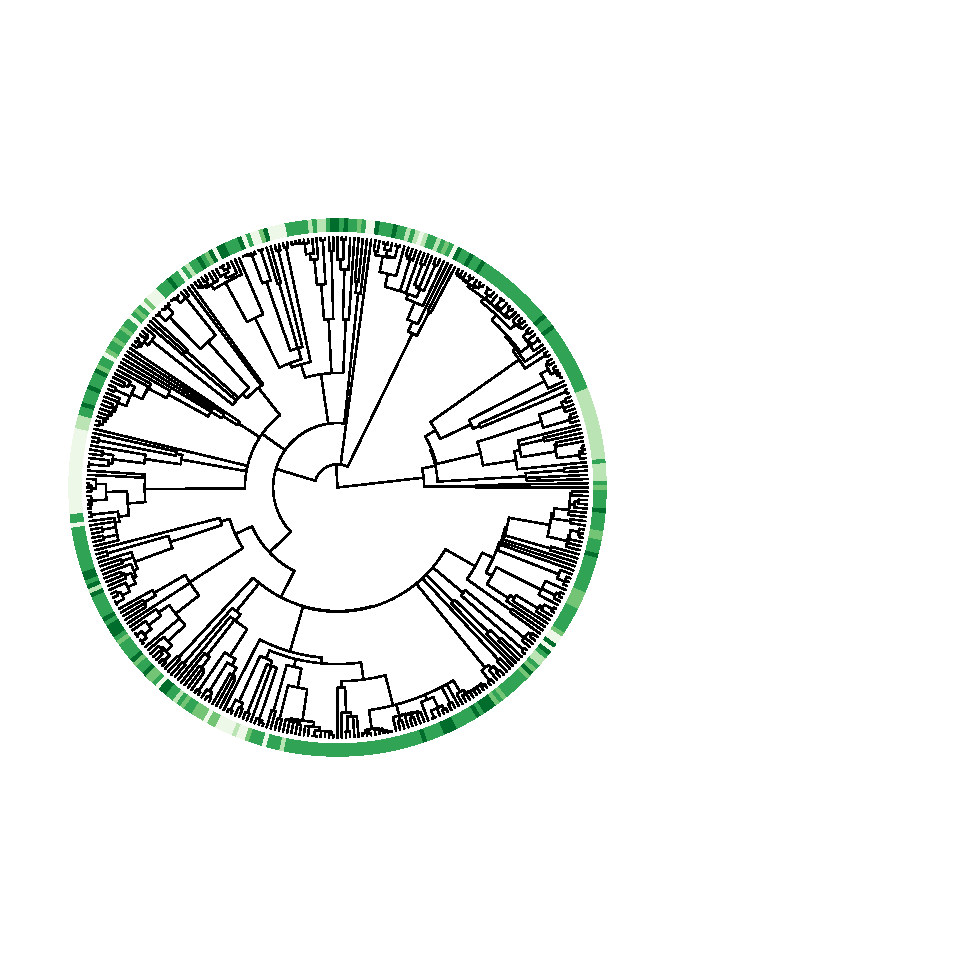
\includegraphics[width=\textwidth]{figures/figure_phylo.pdf}}
\caption{CAPTION} 
\label{fig:phylo}
\end{figure}

\begin{figure}[ht]
\centerline{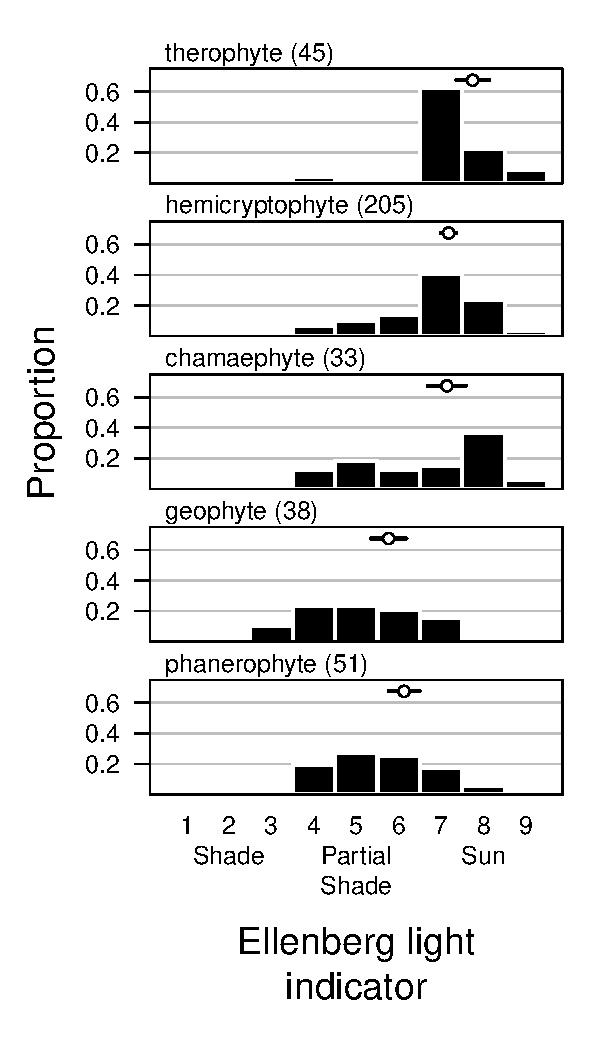
\includegraphics[width=0.5\textwidth]{figures/figure_lf-light.pdf}}
\caption{Lifeforms have different tolerances for sun and shade among British angiosperms. Each panel is the distribution of Ellenberg light indicator values on an integer scale of 1-9 for different Raunki\ae r life forms. Height of the bars indicate the raw proportion of species in each bin for that lifeform. The sample size for each lifeform is listed next in parentheses. The mean (open circle) and 95\% confidence intervals (black line) around the mean Ellenberg light indicator value for each lifeform based on phylogenetic regression are above the histogram.} 
\label{fig:lf-light}
\end{figure}

\begin{figure}[ht]
\centerline{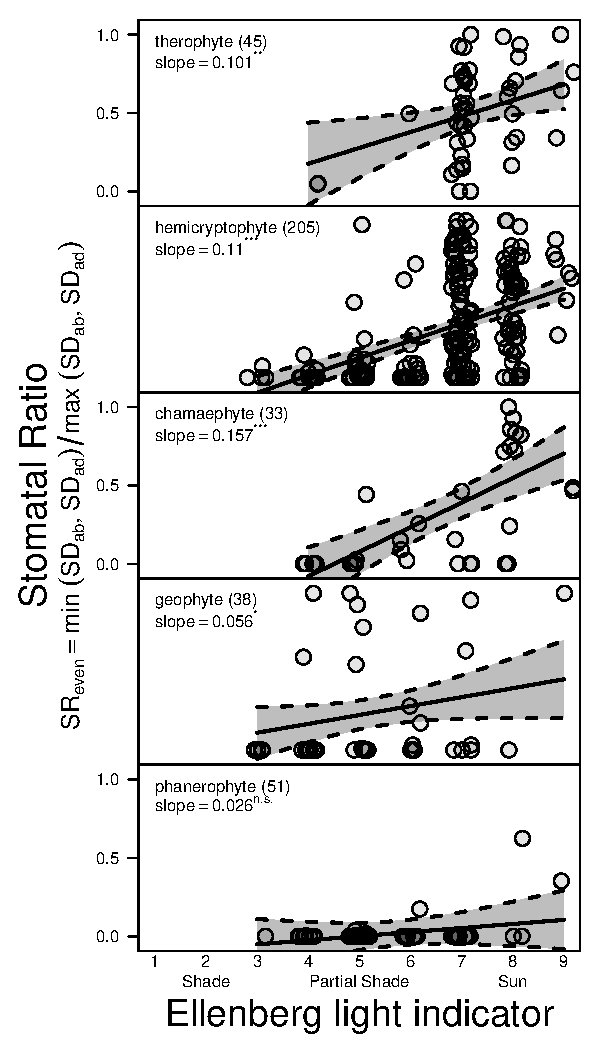
\includegraphics[width=0.5\textwidth]{figures/figure_SRmultReg.pdf}}
%\centerline{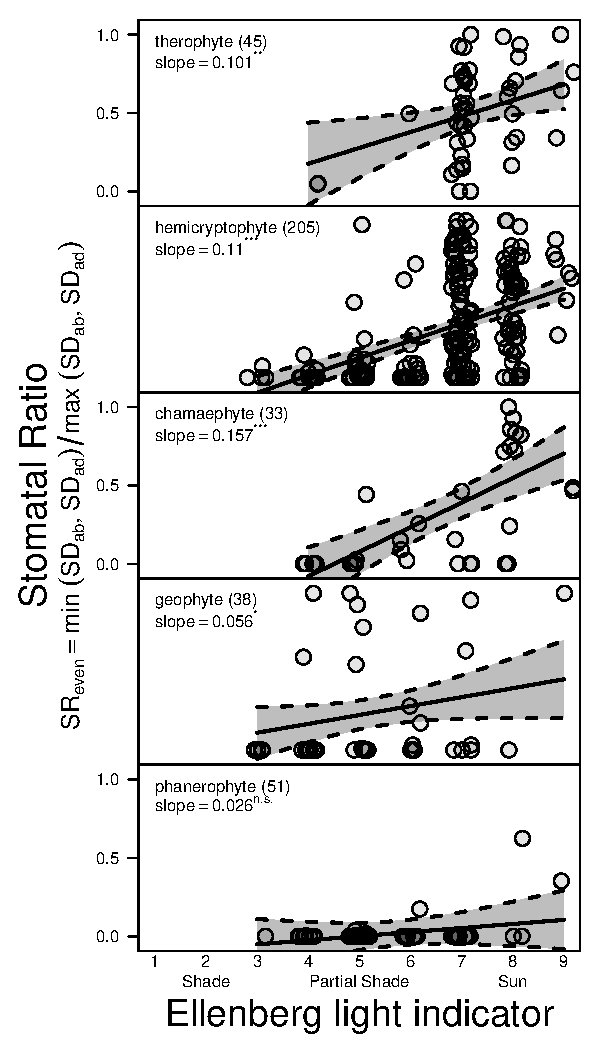
\includegraphics[angle=270]{figures/figure_SRmultReg.eps}} % Needed this to upload file to journal website
\caption{The effect of light on stomatal ratio depends on Raunki\ae r life form. Greater Ellenberg light indicator values (\el) are associated with greater stomatal ratio ($\mathrm{SR_{even}}$) in therophytes, hemicryptophytes, and chamaephytes but not geophytes and phanerophytes. The maximum likelihood slope from phylogenetic regression is given with statistical significance based on 10$^4$ parametric bootstrap samples. Numbers in parentheses next to Raunki\ae r life form are the sample sizes in the final dataset. Estimated slopes (solid line) and 95\% bootstrapped confidence intervals (gray polygon between dashed lines) are plotted against raw data. Points have been jittered for visual clarity.} 
\label{fig:SRmultReg}
\end{figure}

\begin{figure}[ht]
\centerline{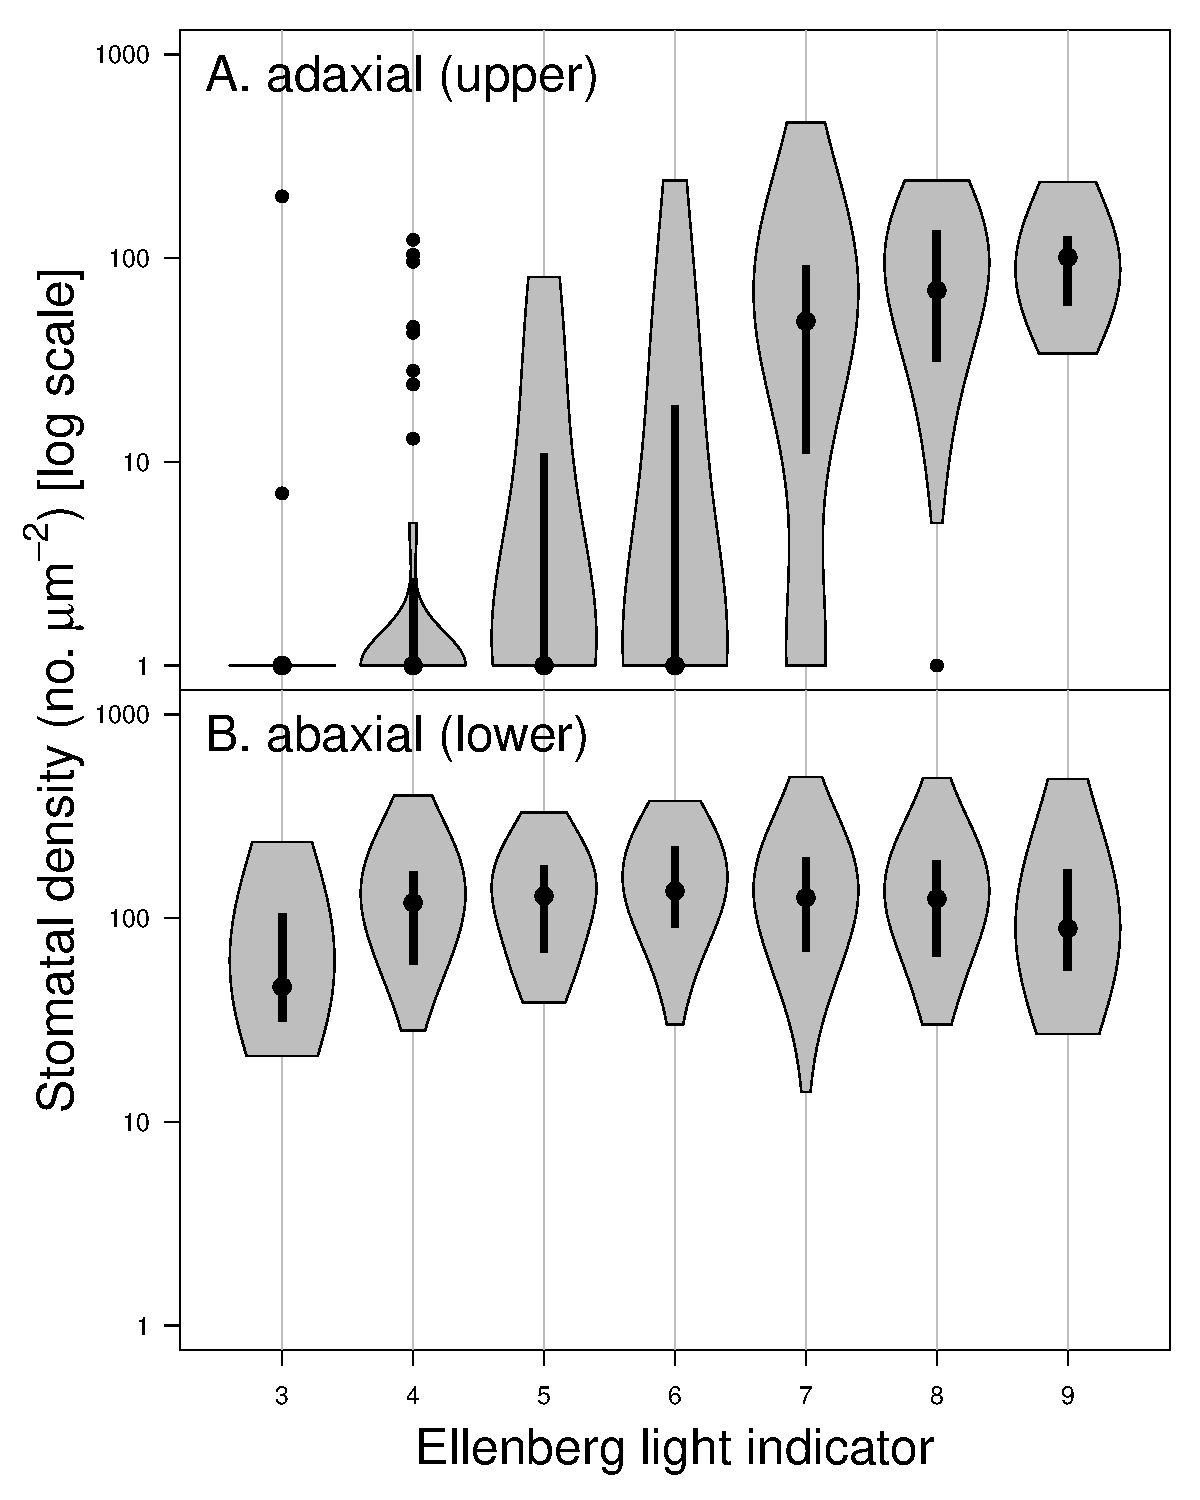
\includegraphics[width=0.5\textwidth]{figures/figure_SD-light.pdf}}
\caption{Light-mediated evolution of stomatal ratio is mostly driven by increased adaxial (`upper') stomatal density (Panel A), whereas abaxial (`lower') stomatal density (Panel B) is similar across Ellenberg light indicator values (\el~$x$-axis). The violin plot shows stomatal density ($y$-axis, log-scale) as a function of \el. The width of the grey polygons indicates the density of data. Length of grey polygon indicate the range of the data; the dot indicates the median; the thick lines indicate the 0.25 and 0.75 quantiles. Points outside the polygons are statistical outliers.} 
\label{fig:SD-light}
\end{figure}

\clearpage

%--------------------------------------------------
% Supporting Information
%--------------------------------------------------

\section*{Supporting Information}

% Modify and restart table/figure numbering for appendixes
\renewcommand\thefigure{S\arabic{figure}}    
\renewcommand\thetable{S\arabic{table}}    
\renewcommand\theequation{S\arabic{equation}}    
\setcounter{table}{0}    
\setcounter{equation}{0}
\setcounter{figure}{0}

%--------------------------------------------------
% Supporting Figures
%--------------------------------------------------

\begin{figure}[ht]
\centerline{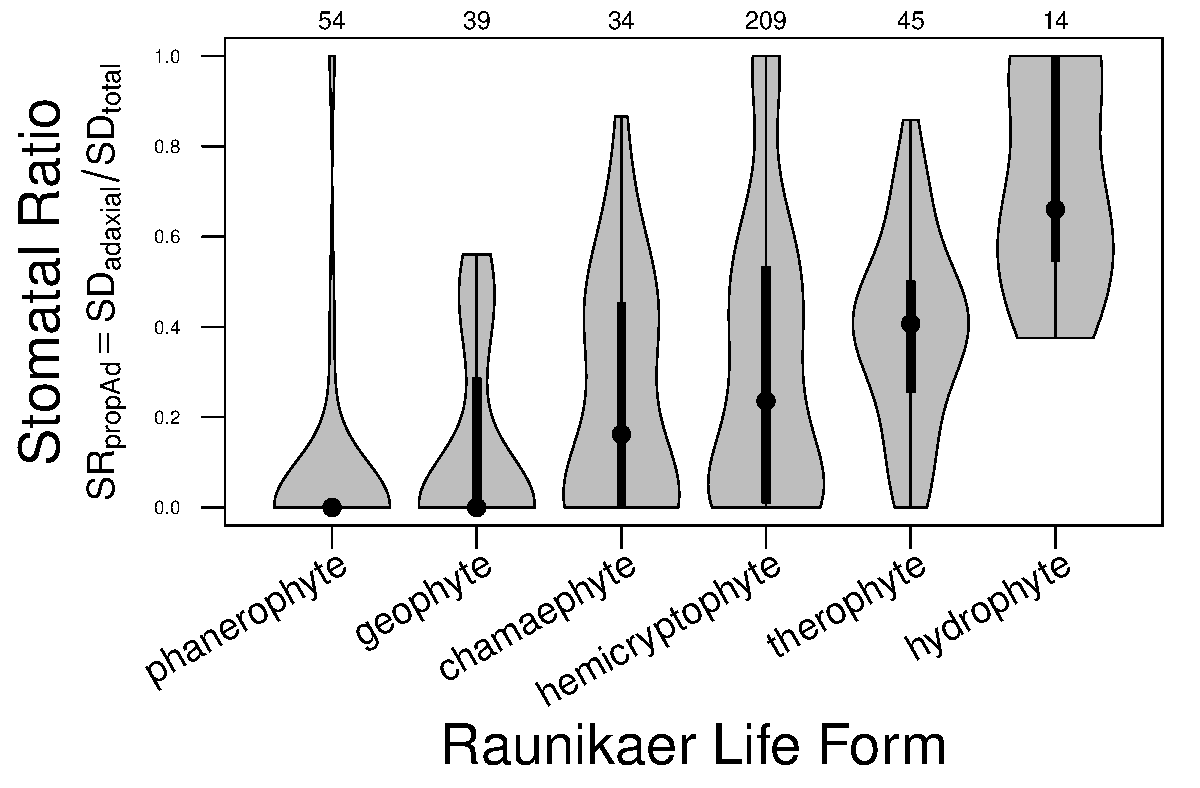
\includegraphics{figures/figureS_violin.pdf}}
\caption{Most hydrophytes are hyperstomatous, having most stomata on the adaxial (`upper') surface (high $\mathrm{SD_{propAd}}$). The violin plot shows stomatal ratio as a function of Raunki\ae r lifeform. The width of the grey polygons indicates the density of data. Length of grey polygon indicate the range of the data; the point indicates the median; the thick lines indicate the 0.25 and 0.75 quantiles. Sample sizes per lifeform in the dataset are given above the upper plot margin. $\mathrm{SD_{ad}}$ and $\mathrm{SD_{total}}$ stand for the stomatal density on the adaxial surface and the total leaf surface (adaxial plus abaxial), respectively.}
\label{fig:violin}
\end{figure}

\end{document}
